\documentclass[
    11pt,
    a4paper,
    egregdoesnotlikesansseriftitles,
    toc=chapterentrywithdots,
    twoside,openright,
    titlepage,
    parskip=half,
    headings=normal,  % reduces heading size
    listof=totoc,
    bibliography=totoc,
    index=totoc,
    captions=tableheading,  % caption below table
    chapterprefix,
    listof=flat,
    final
]{scrbook}


% details about your thesis
\newcommand{\titel}{Abstractive Text Summarization of Meetings}
\newcommand{\artderarbeit}{Bachelorarbeit}  % {Bachelorarbeit,Masterarbeit}
\newcommand{\autor}{Bastian Oppermann}
\newcommand{\studiengang}{Informatik}  % {Informatik,Wirtschaftsinformatik,Medieninformatik}
\newcommand{\matrikelnr}{3068074}
\newcommand{\erstgutachter}{Prof.\,Dr.~Korbinian Riedhammer}
\newcommand{\zweitgutachter}{Prof.\,Dr.~Ngoc\,Thang\,Vu}
\newcommand{\logo}{figures/TH-Nuernberg-RGB.png}
\newcommand{\keywords}{bert, summarization}
 

% custom head and foot
\usepackage[automark]{scrlayer-scrpage}
\pagestyle{scrheadings}
\ihead{\headmark}
\chead{}
\ohead{\pagemark}
\renewcommand*\chaptermarkformat{\chapappifchapterprefix{\ }% 
  \thechapter.\enskip}

\RedeclareSectionCommand[tocindent=0pt]{section}
\RedeclareSectionCommand[tocindent=0pt]{subsection}
%\RedeclareSectionCommand[tocnumwidth=70pt]{chapter}

\usepackage{scrhack}

% other packages
\usepackage[utf8]{inputenc}
\usepackage[T1]{fontenc}
\usepackage{lmodern,relsize,textcomp,csquotes}
\usepackage{amsmath,amsfonts}
\usepackage[ngerman,english]{babel}  % flip for German thesis
\usepackage[final]{graphicx}
\usepackage{setspace,geometry,xcolor}
\usepackage{makeidx}
\usepackage{paralist,ifthen,todonotes}
\usepackage{url}
\usepackage{pdfpages}

% table setup
\usepackage{longtable}
\usepackage{array}
\usepackage{ragged2e}
\usepackage{lscape}

% pdf hyperref
\usepackage[
    bookmarks=true,
    bookmarksopen=true,
    bookmarksnumbered=true,
    bookmarksopenlevel=1,
    pdftitle={\titel},
    pdfauthor={\autor},
    pdfcreator={\autor},
    pdfsubject={\titel},
    pdfkeywords={\keywords},
    pdfpagelabels=true,
    colorlinks=true,
    linkcolor=red,
    urlcolor=magenta,
    anchorcolor=black,
    citecolor=cyan,
    filecolor=magenta,
    menucolor=red,
    plainpages=false,
    hypertexnames=true,
    linktocpage=true,
]{hyperref}


% configure your listings style
\usepackage{listings}
\lstset{
	tabsize=3,
	extendedchars=true,
	frame=single,
	showstringspaces=true,
	numbers=left,
	numberstyle=\small,
	breakautoindent=true
}

% page setup
% \setlength{\topskip}{\ht\strutbox}
\geometry{paper=a4paper,left=2.5cm,top=3.0cm,bindingoffset=.8cm}
\onehalfspacing
\frenchspacing
\clubpenalty = 10000
\widowpenalty = 10000 
\displaywidowpenalty = 10000

% some commands
\newcommand{\ua}{\mbox{u.\,a.\ }}
\newcommand{\zB}{\mbox{z.\,B.\ }}
\newcommand{\dahe}{\mbox{d.\,h.,\ }}
\newcommand{\bzw}{\mbox{bzw.\ }}
\newcommand{\bzgl}{\mbox{bzgl.\ }}
\newcommand{\eg}{\mbox{e.\,g.\ }}
\newcommand{\ie}{\mbox{i.\,e.\ }}
\newcommand{\wrt}{\mbox{w.\,r.\,t.\ }}
\newcommand{\etal}{\mbox{\emph{et.\,al.\ }}}


% TODO remove if not needed...
\usepackage{blindtext}


\begin{document}

\setcounter{secnumdepth}{3}  % numerate subsections
\setcounter{tocdepth}{2}  % ...but don't include them in toc

\frontmatter
\thispagestyle{empty}
\pdfbookmark[1]{Cover}{cov}
\begin{titlepage}

\begin{center}


\includegraphics[width=\linewidth]{figures/TH-Nuernberg-RGB.png}\\[1cm]
\LARGE{Fakultät Informatik}\\[2cm]

\huge
\textbf{\titel}\\[1cm]
%
\Large
\artderarbeit~im Studiengang \studiengang\\[1cm]
%
\large
vorgelegt von

\Large
\autor\\[0.5cm]
\small
Matrikelnummer \matrikelnr\\[2cm]

\vspace*{\fill}

\large
\begin{tabular}{p{3cm}p{8cm}}\\
Erstgutachter:  & \quad \erstgutachter\\[1.2ex]
Zweitgutachter: & \quad \zweitgutachter
\end{tabular}
\end{center}

\begin{center}
\copyright\,\the\year
\end{center}

\vspace{-0.5cm}
\singlespacing
\small
\noindent Dieses Werk einschließlich seiner Teile ist \textbf{urheberrechtlich geschützt}.
Jede Verwertung außerhalb der engen Grenzen des Urheberrechtgesetzes ist ohne Zustimmung des Autors unzulässig und strafbar.
Das gilt insbesondere für Vervielfältigungen, Übersetzungen, Mikroverfilmungen sowie die Einspeicherung und Verarbeitung in elektronischen Systemen.

\end{titlepage}
\cleardoublepage

% download the following form and complete it (hit save in your editor)
% https://intern.ohmportal.de/fileadmin/Gelenkte_Doks/Abt/SZS/SB/SB_0050_FO_Pruefungsrechtliche_Erklaerung_und_Erklaerung_zur_Veroeffentlichung_der_Abschlussarbeit_public.pdf
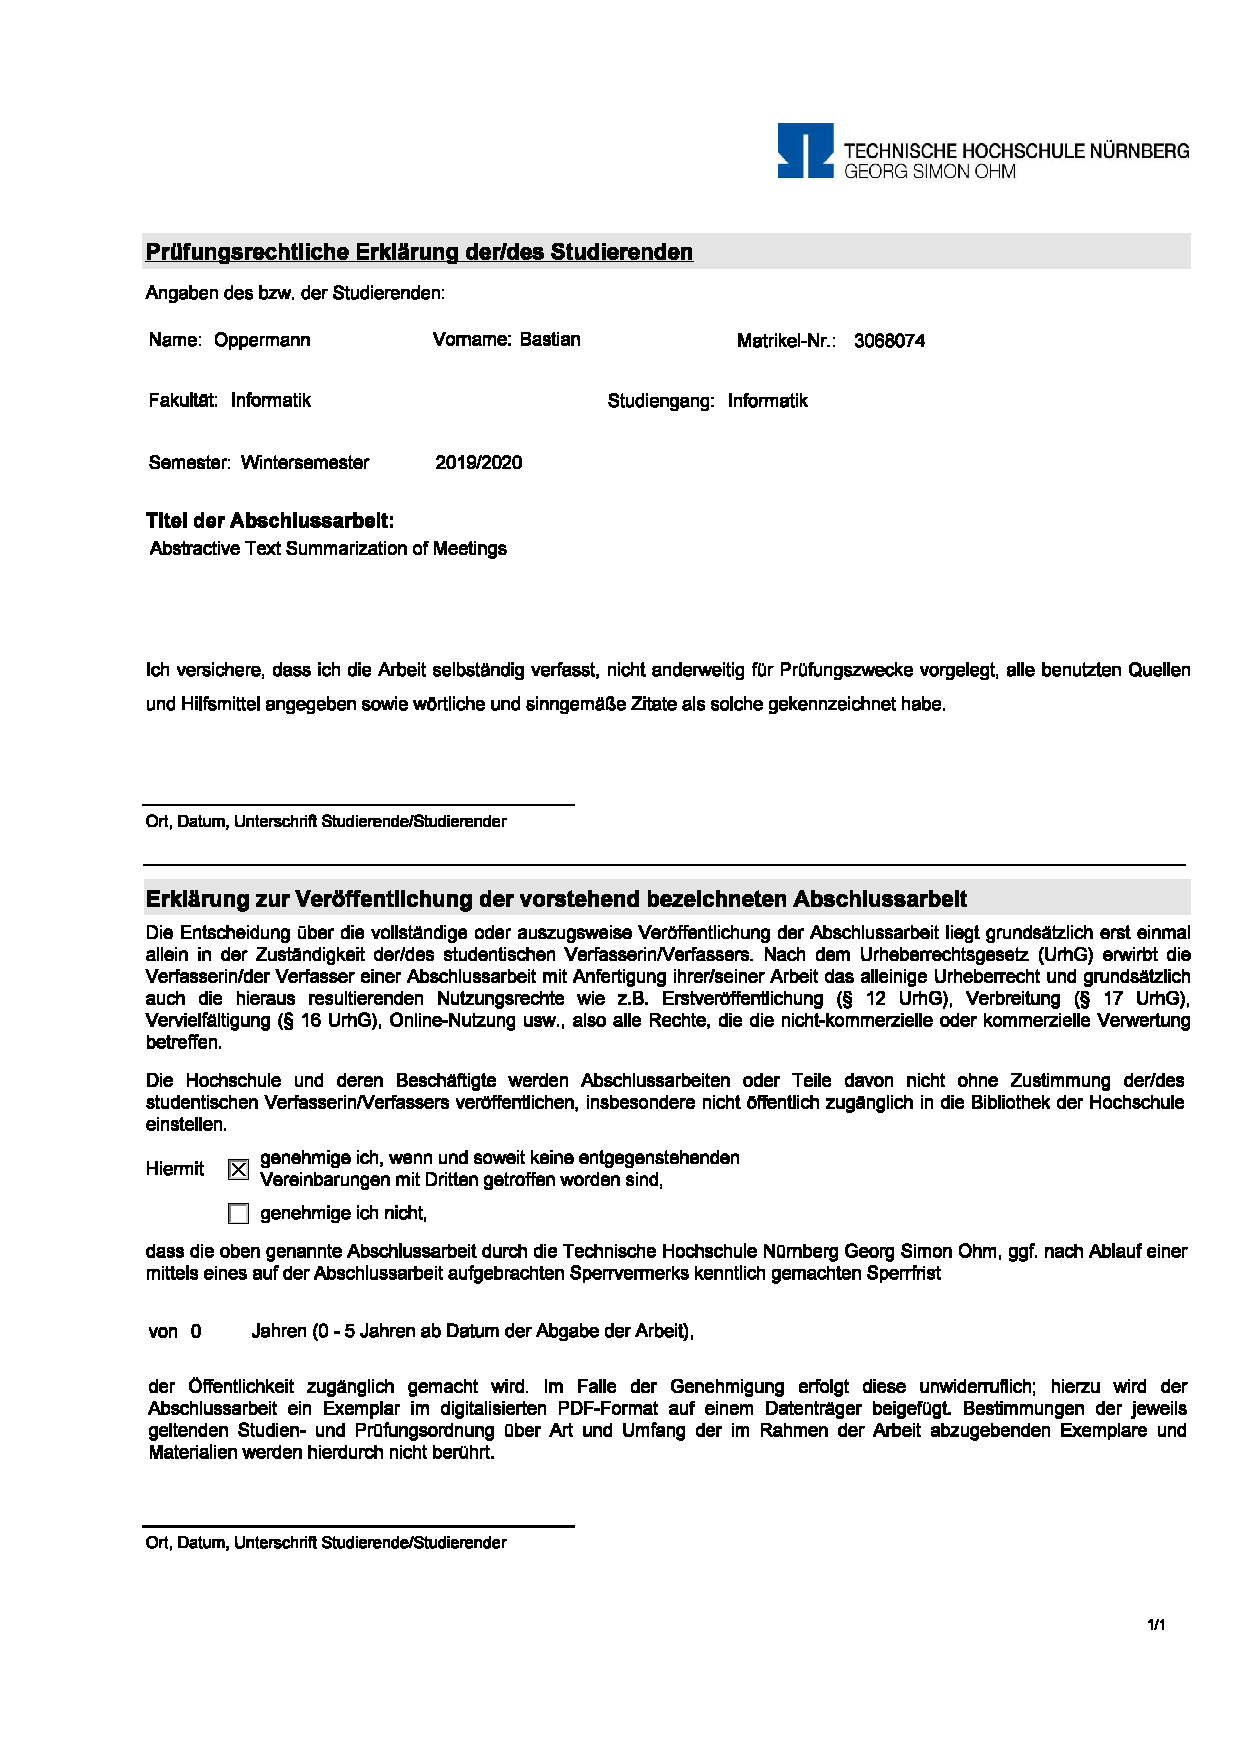
\includepdf{SB_0050_FO_Pruefungsrechtliche_Erklaerung_und_Erklaerung_zur_Veroeffentlichung_der_Abschlussarbeit_public.pdf}\cleardoublepage

\thispagestyle{empty}
\section*{Kurzdarstellung}
\label{sec:kurzdarstellung}

Die vorliegende Bachelorarbeit untersucht, wie ein modernes vortrainiertes neuronales Netz, wie z.B. Googles BERT \cite{devlin2018bert}, zur abstrakten Textzusammenfassung von Meetings genutzt werden kann.

Im Rahmen dieser Arbeit wird ein Tranformer Netz \cite{1706.03762} implementiert, das BERT als seinen Encoder nutzt.
Der Decoder des Netzes ist ein normaler, nicht vortrainierter, Transormer-Decoder.
Das Netz wird hierfür mit Daten aus dem AMI Meeting Corpus \cite{Mccowan05theami} und dem ICSI Meeting Corpus \cite{Janin} trainiert.
Es wird dafür ein 2-stufiges Verfahren genutzt.
Im ersten Schritt wird das Netzwerk darauf trainiert, eine Menge von Dialogen auf einen einzelnen Satz abzubilden, der aus der abstrakten Zusammenfassung des Meetings stammt.
Im zweiten Schritt werden die Meetings nach Themen aufgeteilt und anschließend alle Dialoge eines Themas als Eingabe für das neuronale Netz genutzt.
Die zusammengehängte Ausgabe des Netzes für alle Themen eines Meetings ist dann die fertige Zusammenfassung des gesamten Meetings.
Dies dient zum einen dazu, den benötigten Speicherbedarf von BERT bei langen Textsequenzen zu reduzieren.
Zum anderen kann damit auch das Problem umgangen werden, dass BERT nur mit Textsequenzen bis zu einer Länge von 512 vortrainiert wurde \cite[p.~13]{devlin2018bert}.

Die Arbeit zeigt, dass ein datengetriebener Ansatz in der Theorie funktioniert.
Allerdings haben die Ergebnisse eine sehr starke Neigung dazu, Informationen aus den Traingsdaten in die Zusammenfassung einfliesen zu lassen, selbst wenn diese nicht in der Eingabe vorhanden sind.
Dies ist besonders offensichtlich, wenn ein Netz, das nur mit dem AMI Korpus trainiert wurde, auf den ICSI Corpus angewendet wird.
Die hierbei erziehlten Ergebnisse sind meist sehr schlecht.
Hieraus lässt sich ableiten, dass wesentlich mehr Trainigsdaten notwendig sind, um praxistaugliche Ergebnisse zu erzielen, die unabhängig von einem stark eingegrenzten Kontext, wie es bei den AMI Szenario-Meetings der Fall ist, sind.


\section*{Abstract}
\label{sec:abstract}

This work analyzes how a state-of-the-art pretrained neural network - such as Google's BERT \cite{devlin2018bert} - can be fine-tuned to the task of abstractive text summarization in the context of meetings.

As part of this work a Transformer network \cite{1706.03762} is developed, that uses BERT as its encoder and a plain decoder.
It is trained on the AMI Meeting Corpus \cite{Mccowan05theami} as well as the ICSI Meeting Corpus \cite{Janin}.
To circumvent the high memory usage of BERT at long sequence lengths and the fact that BERT is pre-trained with a maxiumum sequence length of 512 \cite[p.~13]{devlin2018bert}, the summarization is performed using a two-step approach.
First, the network is trained to summarize \(n\) dialouge acts to a single sentence of the meeting's abstractive summary.
Afterwards, a whole meeting is split by its topics and all the dialouge acts of a topic are fed into the trained network as its input.
The concatenated outputs of the Transformer for every topic is the final summary.

The work proofs, that a data-driven approach is feasible in theory.
However, the results have a strong bias towards the context of the meeting and cross-corpus validation on AMI and ICSI shows a very poor performance.
This indicates, that far more training data is necessary for practicable results outside of a very topic-specific context like the scenario meetings of the AMI corpus. \cleardoublepage

\tableofcontents

\mainmatter
\chapter{Introduction}\label{ch:Introduction}

% Motivation

Transfer Learning is known to improve results on many different machine learning tasks.
Google's recently announced language representation model BERT broke records for many Natural Language Processing benchmarks \cite[p.~5--7]{devlin2018bert}, such as  SQuAD v1.1 \cite{rajpurkar-etal-2016-squad} or GLUE \cite{1804.07461}.
There have been some attempts to apply BERT to the problem of abstractive summarization, like \cite{1902.09243} and \cite{1908.08345}.
However, they are usually trained and tested on news articles.
Generating abstractive summaries of meetings is only a rarely researched topic.
Most of the research for summarizing meetings has been focused on either extractive summarization or non Deep Learning approaches such as Dependency Graph Fusion \cite{1609.07035} or Multi-Sentence Compression \cite{shang-etal-2018-unsupervised}.

% ==============
% PROBLEM DEFINITION
% ==============

\section{Problem Definition}

The goal of this work is to analyze, if a data driven approach is feasible for abstractive meeting summarization.
Transfer Learning should be used to compensate for the small amount of training data that is available for meeting summarization.
As BERT's pre-training sequence length of 512 \cite[p.~13]{devlin2018bert} is way shorter than a typical meeting, a method should be developed that deals with this limitation.

% ======
% METHOD
% ======

\section{Method}

As part of this work, a network is developed that uses BERT.
It is trained with data from the two most commonly used meeting corpora, the AMI Meeting Corpus \cite{Mccowan05theami} and the ICSI Meeting Corpus \cite{Janin} that are described in \autoref{ch:used-corpora}.
Cross-corpus validation\footnote{\Eg training on the ICSI corpus and testing on the AMI corpus} is performed to evaluate if the network is able to generalize what it learned.

% =================
% STRUCTURE OF THE WORK
% =================

\section{Structure of the work}

Chapter \ref{ch:theoretical-foundation} explains the theoretical foundation that is necessary for this work.
Chapter \ref{ch:used-corpora} introduces the two used meeting corpora.
Chapter \ref{ch:concept} explains the concept of the model that this works uses.
It will also present how the model is trained.
Chapter \ref{ch:implementation} focuses on the implementation if the model and how the training data is processed.
Chapter \ref{ch:results} presents the results. It shows both the archived scores and provide some hand-picked example outputs.
Chapter \ref{ch:outlook} gives an outlook for possible future research.
Finally, chapter \ref{ch:summary-and-conclusion} summarizes the results of the work and draws a conclusion how they can be interpreted.

\chapter{Data}\label{ch:data}

For this work, two corpora for meeting data are used, the AMI Meeting Corpus \cite{Mccowan05theami} and the ICSI Meeting Corpus \cite{Janin}.

% ==============
% AMI MEETING CORPUS
% ==============

\section{AMI Meeting Corpus}\label{sec:ami-meeting-corpus}

The AMI Meeting Corpus is a corpus for meetings, published by the AMI (Augmented Multi-party Interaction) project in 2006 \cite{Mccowan05theami}.
It contains very detailed annotation of 100 hours of meeting recordings.
The relevant aspects and annotation of the AMI Meeting Corpus, that are relevant for this work, are briefly explained below.

\subsection{Scenario and Non-Scenario Meetings}

The AMI Meeting Corpus contains data for two different types of meetings: Scenario meetings and non-scenario meetings.
For this work, only the data from the scenario meetings are used, as the non-scenario meetings are missing some annotations that are necessary for this work.
The following paragraphs describe the scenario of the scenario meetings.

For the scenario meetings, participants play employees of an electronics company that work together on a project.
They are part of a design team, which tries to develop a prototype for a television remote, because the existing ones are considered not user-friendly, unattractive and old-fashioned.
The participants are assigned one of the following roles:
\begin{itemize}
\item A project manager
\item A marketing expert
\item A user interface designer
\item An industrial designer
\end{itemize}

Each project consists of 4 meetings:
\begin{itemize}
\item A project kick-off meeting
\item A meeting for the functional design of the remote, such as user requirements, technical functionality and the working design
\item A meeting for the conceptual design of the remote's components, such as the materials or the user interface
\item A final meeting to finalize the design and evaluate the results.
\end{itemize}
Before each meetings, the participants perform individual work.

In total, data for 35 of these projects is available, each with the 4 meetings. \cite[p.~2]{Mccowan05theami}

\subsection{Annotations}\label{ssec:ami-annotations}

The following annotations are available and used in this work:

\paragraph{Dialogue Acts}

The transcription of the whole meeting is split into smaller pieces on a per-person basis.
These subsets of the transcription are called "Dialogue Acts".
A dialogue act tries to group word, that belong together to form a speaker's attention, e.g. a question.
Every word of the transcription is part of exactly one dialogue act.
Each dialogue act is classified by its content, but this classification is not used in this work. \cite{amiWebsite}

\paragraph{Topic Segmentation}

Each meeting is split into multiple topics that by themselves may be split into subtopics.
Examples for topics are "industrial designer presentation", "evaluation of prototype" or "project specs and roles of
participants" to name a few. \cite{amiWebsite}

\paragraph{Abstractive Summaries}

\begin{figure}[h]
\begin{lstlisting}[numbers=none]
S1: The project manager introduced the upcoming project to the 
    team members and then the team members participated in an
    exercise in which they drew their favorite animal and
    discussed what they liked about the animal.
S2: The project manager talked about the project finances and
    selling prices.
S3: The team then discussed various features to consider in making
    the remote.
\end{lstlisting}
\caption{Example abstract of abstractive summary for scenario meeting \texttt{ES2002a}.}
\label{fig:abstractive-summary-example}
\end{figure}

For each meeting, abstractive summaries are available.
Each abstractive summary consists of an abstract, decisions, problems/issues and actions, but this work is only using the abstract.
Usually, the abstract consists of multiple sentences.
An example for such an abstract with 3 sentences is shown in \cref{fig:abstractive-summary-example}.

Additionally, for each sentence of the abstractive summary, one or more dialogue acts are selected, that are linked together.
This mapping of $n$ dialogue acts to $1$ sentence of the summary is later used for training, as described in \label{sec:concept-training} in more detail. \cite{amiWebsite}

\subsection{Segmentation of the Corpus}\label{ssec:ami-segmentation-of-the-corpus}

\begin{table}[h]
\centering
\begin{tabular}{@{}ll@{}}
\toprule
\multicolumn{1}{c}{Set} & \multicolumn{1}{c}{Time} \\ \midrule
Training & $\sim$50 hours \\
Development & $\sim$11 hours \\
Test & $\sim$11 hours \\ \bottomrule
\end{tabular}
\caption[Distribution of meeting time of train, dev and test sets]{Distribution of meeting time of train, dev and test sets \cite{amiWebsite}.}
\label{tab:meeting-time-distribution}
\end{table}

To make results comparable with other works that use the corpus, it is split into training, development and test sets.
For the scenario meetings, the data distribution is shown in \cref{tab:meeting-time-distribution}. \cite{amiWebsite}

% ==============
% ICSI MEETING CORPUS
% ==============

\section{ICSI Meeting Corpus}

The ICSI Meeting Corpus, that contains meetings that were collected at the International Computer Science Institute (ICSI) over a period of three years.
It contains about 72 hours of meeting data. \cite{Janin}
As it has a very similar structure than the AMI Meeting corpus described in \cref{sec:ami-meeting-corpus}, this chapter will only focus on their differences that are relevant for this work.

\paragraph{Scenario}

Unlike the scenario meetings of the AMI Meeting Corpus, the ICSI Meeting Corpus are natural meetings that do not have a specific topic.
However, as the meetings are all recorded at the ICSI, they usually follow a specific type.
Because of this, every meeting of the corpus is classified as on one of 5 different meeting types. \cite{Janin}
% TODO Maybe name/describe the 5 types of meetings. But as they are not really important, I will omit them for now...

\paragraph{Topic Segmentation Annotation}

For ICSI, only automatic topic segmentation is available, but no manual segmentation like for AMI.

\paragraph{Segmentation of the Corpus}

Unlike the AMI corpus, the ICSI Meeting Corpus does not come with a predefined split for training, development and test sets.
Because of this missing split, this work will mainly work with the AMI Meeting Corpus and only use the ICSI Meeting Corpus for cross-corpus-validation.
\chapter{Method}\label{ch:method}

In this chapter, we're actually using some code!

\begin{lstlisting}[language=Python,caption={This is an example of inline listing},captionpos=b]
x = 1
if x == 1:
    # indented four spaces
    print("x is 1.")

\end{lstlisting}

You can also include listings from a file directly:

\lstinputlisting[language=Python,caption={This is an example of included listing},captionpos=b]{listings/example.py}

\chapter{Experiments}\label{ch:experiments}

\Blindtext

\chapter{Outlook}\label{ch:outlook}

\Blindtext

\chapter{Summary}\label{ch:summary}

\Blindtext


% remove if not needed
\appendix
\chapter{Supplemental Information}\label{app:supplemental-information}

\Blindtext



\backmatter
\listoffigures
\cleardoublepage

\listoftables
\cleardoublepage

\renewcommand{\lstlistlistingname}{List of Listings}  % change for German thesis
\lstlistoflistings
\cleardoublepage

\bibliographystyle{wmaainf}
\bibliography{refs}

\end{document}
